% !TEX root = ../main.tex
\chapter{Principles of Spectroscopy}
\label{chapter_spectroscopy}
%-------------------------------------------------------------------------------
%	SECTION 1: INTRODUCTION TO SPECTROSCOPY
%-------------------------------------------------------------------------------

\section{Fundamentals of Spectroscopy}
\label{sec:spectroscopy_fundamentals}

\todoidea{This chapter should serve as a foundation by emphasizing electronic transitions, nonlinear optics, coherence phenomena, and their relevance to complex (e.g., biological) systems.
Vibrational and other spectroscopies are less relevant for this work, so they should be mentioned but not in detail.}
\todoidea{
Brief motivation: Why spectroscopy is a powerful probe of quantum dynamics.

Distinction between linear and nonlinear optical spectroscopy.

Position of two-dimensional photon-echo spectroscopy (2D PES) within this landscape.

What this chapter provides: the physical and mathematical tools needed for later modeling.
}


\noindent 
Spectroscopy, in its broadest definition, is the study of the interaction between matter and electromagnetic radiation as a function of wavelength or frequency \cite{berman2011principleslaserspectroscopy, mukamel1995principlesnonlinearoptical}.
It provides insights into the composition, structure, and dynamics of physical systems by examining how they absorb, emit, or scatter light. The fundamental principle underlying all spectroscopic methods is that each atom, molecule, or complex system has a unique set of energy levels, and transitions between these levels involve the absorption or emission of photons with specific energies \todoref{find better source}\cite{boyd2008chapter1nonlinear}. Thats why spectroscopy is a powerful probe of quantum dynamics.



\subsection{Basic Principles}
\label{subsec:basic_principles}

\noindent The foundation of spectroscopy rests on the quantization of energy in atomic and molecular systems. According to quantum mechanics, atoms and molecules can exist only in discrete energy states \cite{albashetal2012quantumadiabaticmarkovian}. The energy difference between two states, $\Delta E$, determines the frequency $\nu$ or wavelength $\lambda$ of light that can be absorbed or emitted during a transition between these states, following Planck's relation:

\begin{equation}
	\Delta E = h\nu = \frac{hc}{\lambda}
	\label{eq:planck_relation}
\end{equation}

\noindent 
where $h$ is Planck's constant and $c$ is the speed of light. The energy structure of matter can thus be probed by observing the spectrum of absorbed or emitted radiation.


%-------------------------------------------------------------------------------
%   NEW SUBSECTION: CHARACTERIZATION OF ELECTROMAGNETIC RADIATION
%-------------------------------------------------------------------------------
\subsection{Characterization of Electromagnetic Radiation}
\label{subsec:em_radiation_characterization}

\noindent 
A monochromatic electromagnetic plane-wave in free space (vacuum) can be written as

\begin{equation}
	E(\vec{r},t) = E_0 \cos(\vec{k} \cdot \vec{r} - \omega t + \phi)
	\label{eq:plane_wave}
\end{equation}

\noindent 
where $E_0$ is the (real) amplitude, $\phi$ a phase-kick, $\vec{k}$ the wavevector (spatial angular frequency), and $\omega$ the angular frequency of the wave. The real field can be decomposed into complex positive and negative frequency parts as

\iffalse
\begin{equation}
	E^{(+)} = E_0 e^{i(\vec{k} \cdot \vec{r} - \omega t + \phi)}
	\label{eq:positive_frequency_e_field}
\end{equation}

\noindent 
with $E^{(-)} = E^{(+)}^{*}$ and thus $E = 1/2 \{E^{(+)} + E^{(-)}\}$.
$E^{(+)}$ is called the positive-frequency part because in Fourier space it contains only components with frequencies $\omega > 0$ \todoref{fact check}. This will come in handy applying a rotating wave approximation as the positive field part rotates in the same direction as the rotating frame and the negative rotates in the opposite direction \cite{hamm2005principlesnonlinearoptical}.
\fi
\noindent 
The fundamental kinematic relations for propagation in vacuum are

\begin{equation}
	\omega = 2\pi\nu, \qquad |\vec{k}| = \frac{2\pi}{\lambda}, \qquad \lambda = \frac{c}{\nu} = \frac{2\pi c}{\omega}
	\label{eq:wavelength_frequency_relation}
\end{equation}

\noindent 
with $\nu$ the (cycle) frequency in hertz (Hz), $\lambda$ the wavelength. 
%In a material medium the phase velocity is $v_p = c/n(\nu)$ and $\lambda$ is replaced by $\lambda_n = v_p/\nu = \lambda/n(\nu)$, where $n(\nu)$ is the refractive index.

\noindent 
Note that the \emph{magnitude of the wavevector } $k = 2\pi/\lambda$ (units m$^{-1}$), shall not be confused with the \emph{(spectroscopic) wavenumber} $\tilde{\nu}$, defined as

\begin{equation}
	\tilde{\nu} = \frac{1}{\lambda} \quad [\mathrm{cm}^{-1}].
	\label{eq:wavenumber_definition}
\end{equation}

This quantity is commonly used in spectroscopy to avoid large powers of ten. 
Now to give a broad idea of where transitions that one would like to probe with spectroscopy lie, we can look at the typical energy scales of different types of transitions.

\subsection{Classification of Spectroscopic Techniques}

\noindent
Spectroscopy can be categorized by (i) the nature of the transition (rotational, vibrational, electronic, nuclear), (ii) the number of photons involved (linear vs.\ nonlinear), and (iii) the detection scheme (absorption, emission, or scattering). 

\noindent
(i):

\noindent
Different types of transitions are probed at distinct regions of the electromagnetic spectrum, reflecting the corresponding energy and time scales and providing fundamentally different information about the system of interest. 

\noindent
Ultrafast laser development has enabled femtosecond and even attosecond spectroscopy, allowing real-time tracking of electron motion and energy flow in complex systems.

\noindent
For example, rotational transitions lie in the microwave region. Here molecular geometry is revealed through quantized rotational energy levels. In vibrational spectroscopy, bonding patterns are measured within the infrared ($\lambda\!\sim\!2.5$–$25\,\mu\mathrm{m}$, $\tilde{\nu}\!\sim\!400$–$4000\,\mathrm{cm^{-1}}$) region of the spectrum. In this thesis electronic transitions between molecular orbitals will be probed with visible frequencies of  ($\lambda\!\sim\!400$–$750\,\mathrm{nm}$, $\tilde{\nu}\!\sim\!13{,}000$–$25{,}000\,\mathrm{cm^{-1}}$), enabling studies of excited-state structure and dynamics.

\noindent
This energetic hierarchy underlies the classification of spectroscopic techniques: higher photon energies probe faster and more localized motions.
While timescales of Micro-milliseconds relate to  Chemical reactions and protein folding, Vibrational relaxation and rotational dynamics happen at picoseconds. Important for this thesis, electronic transitions and vibrational coherences occur at femtoseconds. Recent advances in attosecond spectroscopy now even allow probing real time electron dynamics within atoms and molecules \cite{rupprechtetal2025tracinglonglivedatomic}.

\subsection{Energy Dissipation After Absorption alternative}

\noindent
After an interaction with a laser pulse, absorption of a photon, the excited molecule relax through two principal pathways:
\textbf{Non-radiative relaxation:} Internal conversion and vibrational energy transfer to the environment convert excitation energy into heat. What will be more important for this thesis is \textbf{Radiative relaxation} where the ground state is populated again. The emitted photons that are typically isotropic and thus contribute little to the forward beam.

\noindent
Absorption spectra thus record the net loss of intensity from the incident mode, while emission spectra provide complementary information on excited-state structure and relaxation dynamics. Both will be central in later sections involving heterodyne detection of emitted fields. \todoref{find ref}



\subsection{Macroscopic Samples and Collective Dipolar Oscillations}
\label{subsec:macroscopic_samples}

\noindent 
When considering spectroscopic measurements on macroscopic samples, it is essential to understand how individual molecular responses combine to produce observable signals. In a typical spectroscopic experiment, the sample contains on the order of Avogadro's number ($\sim 10^{23}$) of molecules, each potentially acting as an oscillating electric dipole when interacting with electromagnetic radiation \cite{feynman1965feynmanlecturesphysics}.

\noindent 
The collective behavior of these molecular dipoles determines the induced macroscopic polarization of the sample. When an external electromagnetic field is applied, individual molecules undergo dipole transitions, creating time-varying dipole moments $\vec{\mu}_i(t)$. The coherent superposition of these individual dipolar oscillations produces a macroscopic polarization wave $\vec{P}(\vec{r}, t)$ that can be detected experimentally

\begin{equation}
	\vec{P}(\vec{r}, t) = \frac{1}{V} \sum_{i} \vec{\mu}_i(t) \delta(\vec{r} - \vec{r}_i).
	\label{eq:macroscopic_polarization}
\end{equation}

\noindent 
where $V$ is the sample volume, $\vec{r}_i$ is the position of the $i$-th molecule, and the sum extends over all molecules in the interaction region. This polarization acts as a source term in Maxwell's equations, generating the electromagnetic fields that constitute the spectroscopic signal \cite{abramaviciusetal2009coherentmultidimensionaloptical}

\begin{equation}
	\nabla \times \nabla \times \vec{E}(\vec{r}, t) + \frac{1}{c^2} \frac{\partial^2}{\partial t^2} \vec{E}(\vec{r}, t) = - \frac{4 \pi}{c^2} \frac{\partial^2}{\partial t^2} \vec{P}(\vec{r}, t).
\end{equation}

\noindent
\todoidea{why does it hold that $E_S \propto i P_S$?}

\noindent 
The phase relationships between individual dipolar oscillations are crucial for understanding spectroscopic line shapes and signal intensities \todofix{why?} . 

\todoidea{add the following to a different section / into the results}
In the case of inhomogeneously broadened systems, different molecules oscillate at slightly different frequencies due to variations in their local environment. The resulting dephasing of individual oscillators leads to the characteristic decay of macroscopic coherences observed in techniques such as photon echo spectroscopy \cite{mukamel1995principlesnonlinearoptical}.



\noindent
Now that we have introduced the most important quantity in spectroscopy Eq. \ref{eq:macroscopic_polarization}, we can discuss how it depends on the incident electric field. This leads to linear and nonlinear optics.

%----------------------------------------------------------------------------------------
%	SECTION 2: NONLINEAR OPTICS
%----------------------------------------------------------------------------------------
\section{Nonlinear Optics}
\label{sec:nonlinear_optics}
\todoidea{typically at high field intensities, the response of the medium becomes nonlinear.}
\todoidea{explain Response theory as the standard way to deal with this -> it is a perturbative approach -> mine is numerical and better cite leszczynskietal2017handbookcomputationalchemistry, the most modern one is loaizaetal2025nonlinearspectroscopygeneralized}


In general, the polarization can be expressed as a power series in the electric field:

\begin{equation}
	\vec{P} = \varepsilon_0 (\chi^{(1)} \vec{E} + \chi^{(2)} \vec{E} \cdot \vec{E} + \chi^{(3)} \vec{E} \cdot \vec{E} \cdot \vec{E} + \ldots)
	\label{eq:nonlinear_polarization}
\end{equation}

\noindent 
where $\varepsilon_0$ is the vacuum permittivity and $\chi^{(i)}$ is the $i$-th-order nonlinear susceptibility tensors. 
In the linear regime, the induced polarization $\vec{P}$ can be cut after the first contribution, which is directly proportional to the applied electric field $\vec{E}$.
This relationship describes phenomena such as refraction and absorption.
The higher-order terms give rise to a variety of nonlinear optical phenomena \cite{boyd2008contents}.

\noindent 
\todoidea{this is not so important for this thesis, so keep it short:}
Second-order nonlinear processes, governed by the $\chi^{(2)}$ term, occur only in noncentrosymmetric materials, which lack inversion symmetry \cite{rao2018overviewsecondthird,boyd2008chapter1nonlinear}.  Second-order nonlinear processes include Second Harmonic Generation (SHG), where two photons of frequency $\omega$ combine to generate a photon of frequency $2\omega$; Sum Frequency Generation (SFG), where two photons of frequencies $\omega_1$ and $\omega_2$ combine to produce a photon of frequency $\omega_1 + \omega_2$; Difference Frequency Generation (DFG), where two photons interact to create a photon of frequency $\omega_1 - \omega_2$.


\subsection{Third-Order Nonlinear Processes}
\label{subsec:third_order}

\noindent
Going to third-order, nonlinear processes can occur in all materials, regardless of symmetry \cite{hamm2005principlesnonlinearoptical}. Key third-order nonlinear processes include Third Harmonic Generation (THG), where three photons combine to generate a photon of tripled frequency; Nonlinear Refraction, where the refractive index depends on light intensity, known as the Kerr effect; and Two-Photon Absorption (TPA), which involves the simultaneous absorption of two photons to excite a transition.
The most important third-order process for this thesis is Four-Wave Mixing (FWM) \cite{boyd2008chapter6nonlinear}. Here, three incident and one generated photon interact in a way that satisfies energy conservation $\mathbf{k}_S = \mathbf{k}_1 + \mathbf{k}_2 + \mathbf{k}_3$ generating photon echo signals and allowing for 2D spectroscopy. This will be discussed in detail in the section \ref{sec:phase_matching}.

\noindent
Now that we have a understanding of nonlinear optics, we can discuss how to calculate the nonlinear polarization in practice. The standard way is to use response functions, which will be discussed in the next section.


\section{Light matter interaction - Calculation of the Polarization}
\label{sec:response_functions}

\noindent
The startpoint for this will be the semiclassical Hamiltonian of a quantum mechanically modeled matter-system interacting with classical radiation field described with vector and scalar potentials \todofix{fix this sentence (and) or add the full Hamiltonian}.
Standard textbooks like \cite{garrisonchiao2008quantumoptics,gerryknight2024introductoryquantumoptics} go into the dipole approximation, where the Hamiltonian takes the form

\begin{equation}
	H = H_0 - \mathbf{\hat{\mu}} \cdot \mathbf{E}(t).
\end{equation}

\noindent
Here we remember the electrical field from Eq. \ref{eq:plane_wave} and $\mathbf{\hat{\mu}}$ is the dipole operator of the matter system. This allows us to calculate the macroscopic polarization as the expectation value of the dipole operator

\begin{equation}
	\vec{P}(t) = \langle \mathbf{\hat{\mu}}(t) \rangle = \mathrm{Tr}[\mathbf{\hat{\mu}} \rho(t)]
	\label{eq:polarization_expectation_value}
\end{equation}

\noindent
Similar to the electric field in Eq. \eqref{eq:plane_wave} also the polarization can be decomposed into positive and negative frequency components. For the spectroscopic measurements the positive frequency part is relevant as the emitted signal field is proportional to it \todoref{IS THIS TRUE??} \cite{mukamel1995principlesnonlinearoptical}


\noindent
Now to isolate the effect of a third order non-linear process, we only have to calculate the quantity Eq. \eqref{eq:polarization_expectation_value} for that specific order.
To do that one could also treat the density matrix as an object to do Pertubation theory. This leads to the framework of Response functions. 

\noindent
The following equatons are taken for the optical case of taking the dipole operator as the observable $A = \hat{\mu}$, with the dipole approximation Hamiltonian, but generally they hold for other observable as well, just producing different expectation values. \todoimp{<- find examples?}
The $i$-th order polarization can be written as the convolution of $i$ electric fields \cite{hamm2005principlesnonlinearoptical}

\begin{align}
	P^{(i)}(t) &= \int_{0}^{\infty}\! dt_{i} \int_{0}^{\infty}\! dt_{i-1} \cdots \int_{0}^{\infty}\! dt_{1} \notag \\
	&\quad E\bigl(t-t_{i}\bigr)\, E\bigl(t-t_{i}-t_{i-1}\bigr)\,\cdots\, E\bigl(t-t_{i}-\cdots - t_{1}\bigr) \notag \\
	&\quad S(t_{i},t_{i-1},\ldots,t_{1}),
	\label{eq:response_convolution}
\end{align}

\noindent
where the $i$-th response function is defined as

\begin{equation}
	S^{(i)}(t_{i},\ldots,t_{1})
	\;=\;
	\left(-\frac{i}{\hbar}\right)^{i}
	\Big\langle
	\hat{\mu}(t_{i}+\cdots + t_{1})\;[\hat{\mu}(t_{i-1}+\cdots + t_{1}),\ldots [\hat{\mu}(0),\rho(-\infty)]\ldots]
	\Big\rangle
	\label{eq:response_function_S}
\end{equation}

\noindent
and describes the system's response to $i$ interactions with the electric field.
It was asumed that the interaction takes place at local times $t_i$, and the system is in a equilibrium state (the ground state) before the interaction, at time $t = - \infty$.
It is crucial that the first $i-1$ pulses are inside nested comutators, that represent how these field-interaction drive the system out of equilibrium. The last operator then represents the emitted field and is measured by being traced over the environmental degrees of freedom.

\todoref{fact check this:}
Alternatively Eq. \eqref{eq:response_function_S} can be seen as the $i$-th functional derivative of the expectation value of the dipole operator with respect to the electric field \cite{mukamel1995principlesnonlinearoptical, cho2009twodimensionalopticalspectroscopy}

\begin{equation}
	S^{(i)}(t_i, \dots, t_1) = \frac{\delta \langle \hat{\mu}(t) \rangle}{\delta^i E(t_i) \cdots \delta E(t_1)}  \bigg|_{E=0}.
	\label{eq:response_function}
\end{equation}

\noindent
However this thesis will not go down the path of pertubative calculations, but will instead focus on a more microscopic approach.
Here first the total signal will be calculated, where all pulses are active, well separated in time, and then the desired order will be extracted by filtering out the linear contributions, where only the $i$-th pulse is active.

This way the third order signal can be calculated by 

\begin{equation}
	P^{(3)}(t) = P_{\text{total}}(t) - P^{(2)}(t) - P^{(1)}(t) - P^{(0)}(t)
\end{equation}

\noindent
where the Polarization from Eq. \eqref{eq:polarization_expectation_value} is used. \todofix{actually not true as only the analytical component is extracted, to include phase information.}

\noindent
As mentioned in Sec \ref{subsec:third_order}, FWM is the method discussed in detail. The setup can be seen in Fig. \ref{fig:fwm_box_car_setup}. Here three pulses with wavevectors $\mathbf{k}_1, \mathbf{k}_2, \mathbf{k}_3$ interact with the sample and generate a signal in the direction $\mathbf{k}_S$. 

\begin{figure}[ht]
	\centering
	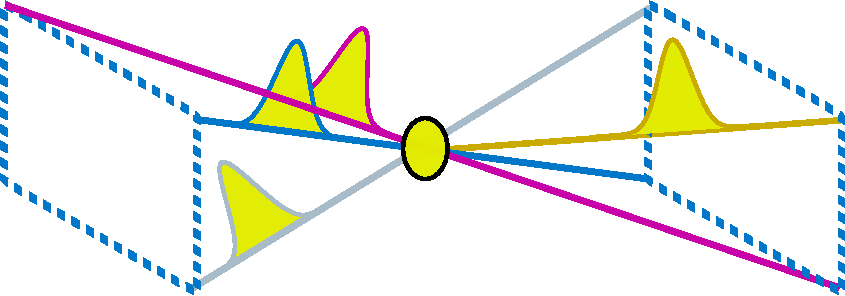
\includegraphics[width=0.8\textwidth]{../figures/FWM_scheme.pdf}
	\caption{Schematic Four-wave mixing setup in a Boxcar geometry. ... \todoimp{Add description. Add S, Add wavevectors, Reduce amplitude of probe pulse.}}
	\label{fig:fwm_box_car_setup}
\end{figure}

\begin{figure}[ht]
	\centering
	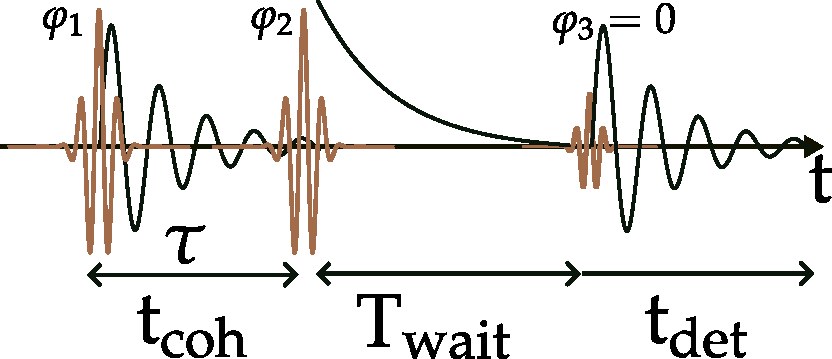
\includegraphics[width=0.8\textwidth]{../figures/FWM_scheme_phase_cycling.pdf}
	\caption{Schematic Four-wave mixing setup. This is the simpler collinear phase-cycling setup, at the cost of requiring multiple measurements with varied pulse phases.
	\todoidea{add ground state at beginning, }}
	\label{fig:fwm_phase_cycling_setup}
\end{figure}

\todoidea{Interaction picture, rotating-wave approximation (introduce but defer justification).}
\todoidea{Also include how to simulate laser pulses:
Gaussian envelope, pulse trains.
1) Time-domain field (carrier × envelope)
$f(t)$ = envelope (e.g. Gaussian $f(t) = \exp\left[-\frac{2\ln 2}{\tau_{\mathrm{FWHM}}^2} t^2\right]$),

$\phi_{\mathrm{CE}}$ = carrier--envelope phase (relevant for few-cycle pulses),

$E_0$ sets peak field (related to pulse energy via the mode area and duration).

Bandwidth for a transform-limited Gaussian:

$\Delta\omega_{\mathrm{FWHM}} \approx \frac{2\ln 2}{\tau_{\mathrm{FWHM}}}$}






\subsection{Heterodyne and Homodyne Detection}
\label{subsec:heterodyne_homodyne}

\noindent There are two main detection schemes used, influencing sensitivity and the information content of the measurements: homodyne and heterodyne detection \cite{abramaviciusetal2009coherentmultidimensionaloptical}.

\noindent In homodyne detection, the intensity of the emitted signal field is measured directly:

\begin{equation}
	S_{\text{HOD}} \propto |E_{\text{S}}|^2 \propto |P^{(3)}|^2
	\label{eq:homodyne}
\end{equation}

\noindent where $E_{\text{S}}$ is the signal electric field and $P^{(3)}$ is the third-order polarization. While experimentally simpler, homodyne detection measures only the signal intensity, losing phase information and it is more susceptible to noise at low signal levels \todoref{find ref}%\cite{abramaviciusetal2009coherentmultidimensionaloptical}.

\noindent Heterodyne detection involves the interference of the signal field with a reference field (local oscillator, LO) of known amplitude and phase:

\begin{equation}
	S_{\text{HET}} \propto |E_{\text{S}} + E_{\text{LO}}|^2 \approx 2\Re{(E_{\text{LO}}^*E_{\text{S}})} + |E_{\text{LO}}|^2 + |E_{\text{S}}|^2
	\label{eq:heterodyne}
\end{equation}

\noindent Since $|E_{\text{LO}}| \gg |E_{\text{S}}|$, the cross-term dominates, and the signal can be extracted by phase-cycling. Heterodyne provides both amplitude and phase information of the signal. The signal scales linearly with the third-order response \todoref{find ref} \todoidea{why is this good?} It also allows for a more direct connection to theoretical models. \todofix{also why?}

\noindent In modern multidimensional spectroscopy, spectral interferometry—a form of heterodyne detection—is widely employed \cite{hybletal1998twodimensionalelectronicspectroscopy}. The signal field and a time-delayed reference pulse are spatially overlapped and spectrally resolved.


\section{Wavevector Phase-Matching Conditions}
\label{sec:phase_matching}

\noindent 
In nonlinear optical processes, multiple light waves interact within a material to generate new frequencies. For these processes to be efficient, the phase relationship between the interacting waves must be maintained throughout the propagation distance. This condition is known as phase-matching.
\noindent 
Like mentioned before, it represents momentum conservation of the incident and outgoing photons. For a general nonlinear process, the wavevector of the generated signal ($\vec{k}_s$) is determined by the vector sum of the input wavevectors:

\begin{equation}
	\vec{k}_s = \pm\vec{k}_1 \pm\vec{k}_2 \pm\vec{k}_3 \pm \ldots
	\label{eq:phase_matching}
\end{equation}

\noindent 
The signs depend on whether the corresponding field acts as a "bra" ($-$) or a "ket" ($+$) in the quantum mechanical description, which corresponds to photon emission or absorption, respectively.

Each laser pulse interacts with the dipole operator $\mu$.
In the rotating-wave approximation (RWA), each field $E_i(t) \propto e^{-i\omega_i t}$ can either:
\todoimp{fact check this:}
Excite the ket side: $\mu_{-} E_i(t) \rightarrow e^{-i\omega_i t} \rightarrow$ forward coherence $e^{-i\omega_{eg} t}$

De-excite the bra side: $\mu_{+} E_i^{*}(t) \rightarrow e^{+i\omega_i t} \rightarrow$ backward (complex-conjugate) coherence $e^{+i\omega_{eg} t}$

That's why the sign in the phase-matching condition ($\pm k_i$) tells you which side of the density matrix the field acted on.

\noindent 
Different combinations of signs correspond to different phase-matching conditions, leading to signals in different spatial directions. These distinct signal directions allow separation of various nonlinear optical processes.


\subsection{Rephasing and nonrephasing Signals}
\label{subsec:rephasing_nonrephasing}

\noindent 
To reduce the number of contributions to the third-order polarization, you can make three vital simplifications: 1.) strict time ordering of the pulses, 2.) the rotating wave approximation (RWA), and 3.) phase-matching \cite{hamm2005principlesnonlinearoptical,  % TODO delete the rest
mukamel1995principlesnonlinearoptical, cho2009twodimensionalopticalspectroscopy, jonas2003twodimensionalfemtosecondspectroscopy}.
For these assumptions, the only surviving terms in the third order polarization are the rephasing and nonrephasing contributions \cite{cho2009twodimensionalopticalspectroscopy, jonas2003twodimensionalfemtosecondspectroscopy}.
\textbf{Rephasing signal} follow the phase-matching condition $\vec{k}_s = -\vec{k}_1 + \vec{k}_2 + \vec{k}_3$. The first interaction creates a coherent superposition between ground and excited states, generated by a complex conjugate interaction of the "bra". The second pulse converts this coherence into a population, and the third pulse generates a new coherence that emits the signal. The phase accumulated due to different frequencies can be reversed during the period between the third interaction and signal emission. This leads to a photon echo effect at $t_{\text{det}} \approx t_{\text{coh}}$ where the dephased components rephase.
This happens for an inhomogeneously broadened ensemble of systems, where different realizations of the system have different transition energies, while the laser pulses drive at constant frequency of $\omega_L$. As a result, some realizations dephase quicker than others. Some realizations should come back in phase around $t_{\text{det}} \approx t_{\text{coh}}$ which is exactly this photon echo.
Contrary to this, \textbf{nonrephasing signal} satisfy $\vec{k}_s = +\vec{k}_1 - \vec{k}_2 + \vec{k}_3$. In this case, the first pulse creates a forward-evolving coherence, and the phase evolution at the third pulse continues in the same direction, and no echo is formed.


\subsection{Phase Cycling in Nonlinear Spectroscopy}
\label{subsec:phase_cycling}

\noindent 
While phase-matching enables the spatial isolation of desired nonlinear Liouville pathways, phase cycling provides an alternative approach by distinguishing signals based on their phases rather than their spatial propagation directions. \todoref{find ref}%\cite{tan2008, yan2009}.
\cite{mukamel1995principlesnonlinearoptical, cho2009twodimensionalopticalspectroscopy, jonas2003twodimensionalfemtosecondspectroscopy, brixneretal2004phasestabilizedtwodimensionalelectronic, greenetal2024vibrationalcoherenceshalfbroadband}.

\noindent 
Here the collinear beam line geometry can be used, simplifying the experimental setup.
This technique is particularly valuable when studying samples without scattering.

\noindent 
And for simulations, as done here, it facilitates the separation of rephasing and nonrephasing signals within the same measurement series.

\noindent 
In phase cycling, multiple measurements are taken with systematically varied phases of the excitation pulses. The desired nonlinear signals can then be extracted through appropriate linear combinations of these measurements. The fundamental principle relies on the fact that different nonlinear pathways respond distinctly to changes in the phases of the input fields.

\noindent 
For a third-order signal generated by three excitation pulses with phases $\phi_1$, $\phi_2$, and $\phi_3$, as seen in Fig. \ref{fig:fwm_phase_cycling_setup}.

\noindent 
By varying the input phases through a complete cycle (in steps of $\pi/2$) and applying discrete Fourier transform to the collected data, specific pathways can be isolated based on their phase dependencies.


\subsection{Phase-Cycling Fourier Selection and Construction of 2D Spectra}
\label{subsec:phase_cycling_fourier_selection}


\noindent 
The nonlinear polarization induced by three incident pulses can be expressed as a Fourier series in the pulse phases $\phi_1, \phi_2, \phi_3$, and individual phase-matched components are isolated via an inverse Fourier transform:

\begin{align}
	P^{(3)}_{n_1,n_2,n_3}(t_{\text{coh}},T,t_{\text{det}}) =
	\frac{1}{(2\pi)^3} \int_{0}^{2\pi}	\int_{0}^{2\pi} \int_{0}^{2\pi}  
	& d\phi_1 d\phi_2 d\phi_3
	e^{-i(n_1\phi_1+n_2\phi_2+n_3\phi_3)} \\
	& P^{(3)}(\phi_1,\phi_2,\phi_3;t_{\text{coh}},T,t_{\text{det}}).
	\label{eq:continuous_phase_cycling}
\end{align}

\noindent 
The physically relevant phase-matching directions correspond to:

\begin{align}
	\vec{k}_{\mathrm{R}}  & = -\vec{k}_1 + \vec{k}_2 + \vec{k}_3,
	                      & (n_1,n_2,n_3)                         & = (-1,+1,+1), \label{eq:rephasing_selection}    \\
	\vec{k}_{\mathrm{NR}} & = +\vec{k}_1 - \vec{k}_2 + \vec{k}_3,
	                      & (n_1,n_2,n_3)                         & = (+1,-1,+1), \label{eq:nonrephasing_selection}
\end{align}

\noindent 
yielding the rephasing (R) and nonrephasing (NR) contributions, respectively.

\noindent 
The (wavevector) phase-matched rephasing signal direction corresponds to selecting the Fourier index triple $(n_1,n_2,n_3)=(-1,+1,+1)$, while the nonrephasing direction corresponds to $(+1,-1,+1)$ \cite{mukamel1995principlesnonlinearoptical, cho2009twodimensionalopticalspectroscopy, greenetal2024vibrationalcoherenceshalfbroadband}.

\noindent 
The emitted field in a given phase-matching direction is proportional to the corresponding polarization:

\begin{equation}
	E_{k_s}(t_{\text{coh}},T,t_{\text{det}}) \propto i P_{\vec{k}_S}(t_{\text{coh}},T,t_{\text{det}}).
	\label{eq:field_polarization_relation}
\end{equation}


\paragraph{Time--Frequency Transforms.}

\noindent 
After phase selection, the third order complex time-domain field $E_{k_S}(t_{\text{coh}}, T, t_{\text{det}})$ is Fourier transformed over the detection time $t_{\text{det}}$ and the coherence time $t_{\text{coh}}$ to construct the two-dimensional spectra (cf. Eq.~\eqref{eq:2des_signal}):

\begin{align}
	S_{R}(\omega_{\text{coh}}, T, \omega_{\text{det}})
	 & =
	\int dt_{\text{coh}} \int dt_{\text{det}} \;
	e^{+ i \omega_{\text{coh}} t_{\text{coh}}} e^{- i \omega_{\text{det}} t_{\text{det}}}
	E_{R}(t_{\text{coh}}, T, t_{\text{det}}),
	\label{eq:rephasing_transform} \\
	S_{NR}(\omega_{\text{coh}}, T, \omega_{\text{det}})
	 & =
	\int dt_{\text{coh}} \int dt_{\text{det}} \;
	e^{- i \omega_{\text{coh}} t_{\text{coh}}} e^{- i \omega_{\text{det}} t_{\text{det}}}
	E_{NR}(t_{\text{coh}}, T, t_{\text{det}}),
	\label{eq:nonrephasing_transform}
\end{align}

\noindent 
where $E(t_{\text{coh}}, T, t_{\text{det}})$ is the time-domain electrical signal field.

\noindent 
The opposite sign in the $t_{\text{coh}}$-exponent implements the standard convention distinguishing rephasing (photon-echo) and nonrephasing contributions \cite{cho2009twodimensionalopticalspectroscopy, greenetal2024vibrationalcoherenceshalfbroadband}. In discrete numerical implementations, Eqs.~\eqref{eq:rephasing_transform}--\eqref{eq:nonrephasing_transform} are approximated by (shifted) fast Fourier transforms \cite{cho2009twodimensionalopticalspectroscopy, greenetal2024vibrationalcoherenceshalfbroadband}.

\paragraph{Global Phase and Absorptive Combination.}

\noindent 
The experimentally measured (or simulated) complex spectra $S_{R}$ and $S_{NR}$ can be combined to  construct the purely absorptive 2D spectrum \cite{mukamel1995principlesnonlinearoptical, jonas2003twodimensionalfemtosecondspectroscopy, greenetal2024vibrationalcoherenceshalfbroadband}
\begin{equation}
	S_{\text{abs}}(\omega_{\text{coh}}, T, \omega_{\text{det}})
	=
	\Re \left\{
	S_{R}(\omega_{\text{coh}}, T, \omega_{\text{det}}) + S_{NR}(\omega_{\text{coh}}, T, \omega_{\text{det}})
	\right\}.
	\label{eq:absorptive_spectrum}
\end{equation}

\noindent 
The absorptive spectra is free from broadening refractive contributions \cite{fullerogilvie2015experimentalimplementationstwodimensional}.



%----------------------------------------------------------------------------------------
%	SECTION 4: PHOTON ECHO SPECTROSCOPY
%----------------------------------------------------------------------------------------
\section{Photon Echo Spectroscopy}
\label{sec:photon_echo}
\noindent 
The echo intensity as a function of the delay time $t_{\text{coh}}$ reveals information about the dephasing processes in the system.

\noindent 
It is important to emphasize that static inhomogeneity is crucial for the appearance of the photon echo signal. This inhomogeneity arises from variations in the local environment of individual quantum systems within the ensemble, leading to a distribution of transition frequencies. In this thesis, in the numerical simulations, static inhomogeneity is taken into account by averaging the results over an ensemble of different realizations of the Hamiltonian \cite{cho2009twodimensionalopticalspectroscopy, mukamel1995principlesnonlinearoptical}. Without this inhomogeneous distribution, all systems would evolve identically, and the characteristic echo phenomenon would not occur.

\noindent 
By scanning the waiting time $T$, this technique allows measurement of population dynamics and spectral diffusion processes.

\subsection{Two-Dimensional Electronic Spectroscopy}
\label{subsec:2d_spectroscopy}

\noindent 
It correlates excitation and detection frequencies, revealing couplings between different transitions and energy transfer pathways.

\noindent 
Recall that a complete 2D spectrum is built from repeated three-pulse sequences while the coherence time $t_{\text{coh}}$ is scanned. The rephasing photon-echo signal arises after a finite rephasing time $t$ for sequences in which pulse 1 precedes pulse 2 ($t_{\text{coh}}>0$) and is recorded in the phase-matched direction $-\vec{k}_1 + \vec{k}_2 + \vec{k}_3$. As discussed in Subsec.~\ref{subsec:rephasing_nonrephasing}, the ground–excited coherences during $t_{\text{coh}}$ and $t$ accumulate opposite phases in the rephasing branch. When the ordering of pulses 1 and 2 is reversed ($t_{\text{coh}}<0$), these phase factors add rather than cancel, yielding a nonrephasing free-induction–decay signal that emerges immediately following pulse 3; this contribution provides information complementary to the rephasing branch \cite{ginsbergetal2009twodimensionalelectronicspectroscopy}.

\noindent The resulting 2D spectrum contains peaks along the diagonal ($\omega_{\text{coh}} = \omega_{\text{det}}$) corresponding to the linear absorption spectrum, while off-diagonal peaks reveal couplings and energy transfer between different states. The evolution of the 2D spectra with waiting time $T$ provides detailed information about energy transfer kinetics, spectral diffusion, and quantum coherence effects.

\subsection{Applications of Photon Echo Spectroscopy}
\label{subsec:echo_applications}

\noindent Photon echo techniques have been applied to a wide range of problems across chemistry, biology, and materials science:

\textbf{Exciton dynamics} in photosynthetic complexes, revealing quantum coherent energy transfer pathways \todoref{find ref}%\cite{engel2007, schlau-cohen2011}
\textbf{Vibrational dynamics} in proteins and liquids, elucidating structural fluctuations and hydrogen-bonding networks \cite{hammzanni2011conceptsmethods2d}
\textbf{Charge transfer processes} in organic photovoltaics and light-harvesting systems
\textbf{Coupling mechanisms} between electronic and vibrational degrees of freedom \cite{khaliletal2004vibrationalcoherencetransfer}



%----------------------------------------------------------------------------------------
\todoidea{

2. Regroup / Change Order
3. Improvements
To make the chapter a stronger foundation, enhance clarity, relevance, and connections to your thesis. Focus on electronic spectroscopy, open quantum systems (e.g., dephasing, dissipation), and biological contexts (e.g., microtubules as complex open systems). Add transitions between sections for better flow.

Add Thesis-Specific Emphasis: Throughout, weave in connections to open quantum systems (e.g., in "Energy Dissipation," link to Lindblad operators or bath interactions). In "Two-Dimensional Electronic Spectroscopy," explicitly state how 2DES reveals couplings and dynamics in systems like microtubules. Add a forward-looking paragraph in the intro/outro noting how this chapter sets up your modeling work.

Improve Mathematical Rigor and Clarity: Equations are good, but add brief explanations of their relevance (e.g., after Eq. 2.1, note how it applies to electronic transitions). For complex sections like phase cycling, use more figures or diagrams (you already have a TODO for one). Ensure notation consistency (e.g., use $\omega$ for angular frequency uniformly).

Enhance Biological Relevance: In "Applications," expand on exciton dynamics in photosynthetic systems as analogs to microtubule coherence. Add a subsection or paragraph on "Towards Biological Systems" at the end, discussing how 2DES can probe quantum effects in cytoskeletal structures.

Strengthen References and Citations: You have many TODOs for refs—prioritize adding them, especially for 2DES and open systems (e.g., cite Mukamel for nonlinear optics, and papers on biological 2DES). Ensure citations align with your thesis's scope.

Improve Flow and Language: Add transitional sentences (e.g., "Building on these fundamentals, we now explore nonlinear optics..."). Use active voice and concise language. Fix minor issues like inconsistent capitalization (e.g., "Rephasing" vs. "rephasing").

Add Figures and Examples: You have a TODO for a figure in phase cycling—add it. Include simple examples (e.g., a toy model of electronic transitions in a two-level system) to illustrate points.

Overall Cohesion: End with a strong conclusion summarizing how these principles underpin your thesis's modeling of microtubules. This reinforces the chapter as a foundation.}